\section{Supporting Information}
\setcounter{figure}{0}
\renewcommand{\thefigure}{S\arabic{figure}}

\subsection{SLAP single-edge ablation and completion}
Binary single-edge sweeps recover 1,785 Golden references and weighted sweeps recover 1,762; their complementary outputs yield 1,795 recoveries in union (\Cref{fig:slap-ablation}). SLAP's initialization is rebuilt after every cut, following the protocol in Methods.

\begin{figure}[htb]
\centering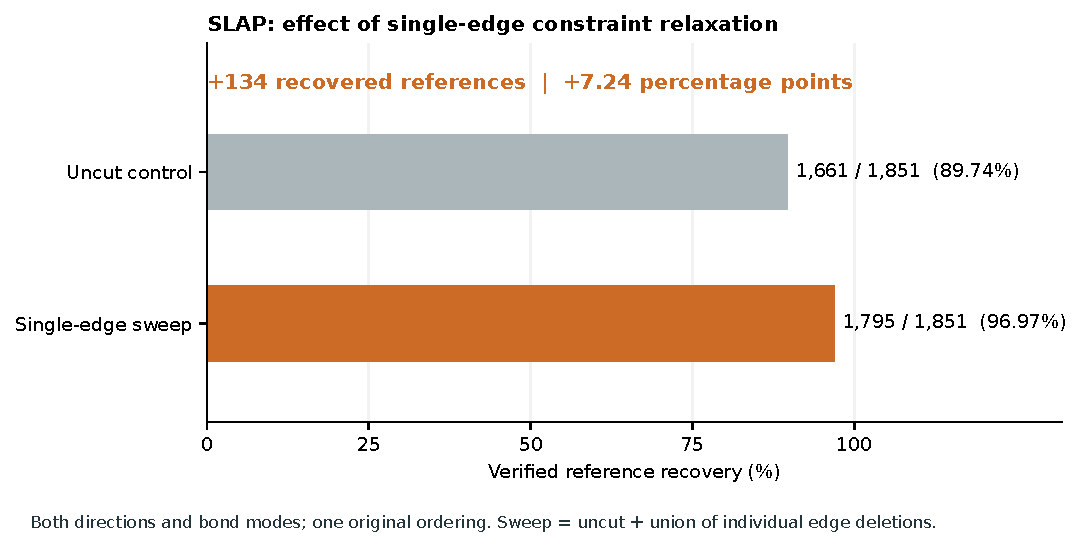
\includegraphics[width=.83\linewidth]{figs/figS1_slap_ablation.pdf}
\caption{\textbf{Supporting single-edge ablation in SLAP.} The control and sweep use the same original ordering, both directions, and binary and weighted modes. The sweep unions the uncut output with outputs from individual source-edge deletions. Recovery increases by 134 cases (7.24 percentage points). All 1,851 records remain in the denominator, including incomplete variants. This experiment evaluates the cut policy in SLAP, not the individual components of GRAFT.}
\label{fig:slap-ablation}
\end{figure}

Of 355,104 planned calls, 352,210 are recorded: 352,208 succeeded and two had upstream exceptions. No returned mapping fails strict format and endpoint-preservation validation. There are 65 watchdog-limited variants among 7,404 case/direction/mode variants; their completed cuts remain included.

Earlier expanded SLAP, with a separate ordering budget, recovers 1,691 (91.36\%). Its union with the new sweep recovers 1,797 (97.08\%), a separate result that is excluded from the ablation figure. Of 54 remaining cases in that union, 50 were fully swept and valid and four were incomplete.

\subsection{Default competitor reproduction}
All 1,851 Golden records were submitted to the released configurations in \Cref{tab:competitors}. These are saved common-evaluator results, not literature numbers. SLAP's first output is not asserted to be a separately ranked top-1. Chython denotes its released ONNX implementation rather than a historical GraphormerMapper checkpoint.

\begin{table}[h]
\centering\small
\caption{\textbf{Released implementations under the common evaluator.} Correctness columns give counts out of 1,851. Output cardinalities and search budgets differ.}
\label{tab:competitors}
\begin{tabular}{lrrr}\toprule
Implementation & First correct & Any correct & Exceptions\\\midrule
RXNMapper 0.4.3 & 1,547 & 1,547 & 0\\
LocalMapper 0.1.5 & 1,605 & 1,605 & 0\\
Chython 2.18 / chython-rxnmap 2.0 & 1,561 & 1,561 & 5\\
SLAPMapper 1.0.0, binary & 1,399 & 1,591 & 0\\
SLAPMapper 1.0.0, weighted & 1,401 & 1,564 & 0\\
Indigo 1.46.0 & 692 & 692 & 133\\
RDT 4.0.0 & 1,030 & 1,030 & 0 after retry\\\bottomrule
\end{tabular}
\end{table}

Indigo returned 503 predictions with duplicate heavy-atom labels and seven with changed endpoint chemistry, in addition to exceptions. Duplicate labels were observed in its native API on an inspected example. The score should not be generalized to historical Indigo benchmarks. Chython returned 29 endpoint-modifying predictions. RDT required worker restart and retry after a JVM failure and broken-pipe cascade; 232 affected initial attempts remain archived. Three final RDT candidates failed validation.

\subsection{Separate experimental versions}
The seed ablation uses \texttt{98b01b1}; the earlier publication run uses \texttt{bb0a7d7}. The former's ten-order evaluation has 1,836 recoveries, five absences, and ten unknowns. The latter has 1,839 recoveries, nine absences, and three unknowns. Similar high-level settings do not establish output equivalence. The earlier run completed 3,689 of 3,702 directional searches; 13 reached the watchdog. Its representative top-5 recovery is 1,789/1,851 (96.65\%), distinct from top-5 family and event-window recovery.

Relative to ten orders, one order no longer verifies cases 44, 602, 850, 912, 1314, 1384, and 1568; 912 is unknown and the other six are absent. Two orders no longer verify 44, 602, 850, 1314, 1384, and 1568; 850 and 1568 are unknown. Both fresh runs verify 1033, 1786, 1799, and 1823, previously unknown. Identifiers are zero-based.

\subsection{Concrete recovery beyond minimum event score: earlier engine}

The earlier publication engine verifies 1,839/1,851 references (99.35\%) bidirectionally, with nine absences and three unknowns. Its representative top-1 result is 1,434/1,851 (77.47\%). This gap illustrates why family recovery cannot be presented as single-answer accuracy.

Extraction from those archives recovers all 1,839 as concrete candidates within six additional bond events of the best collected candidate (\Cref{fig:windows}). At minimum score alone, recovery is 1,692 (91.41\%); allowing two additional events gives 1,817 (98.16\%). This is an event window, not top-$k$. Extraction remains bounded: 20,916 visited families are unresolved and only 409 bidirectional records have exhaustive extraction certificates. The result shows useful higher-event candidates without establishing that all are chemically plausible.

\begin{figure}[tb]
\centering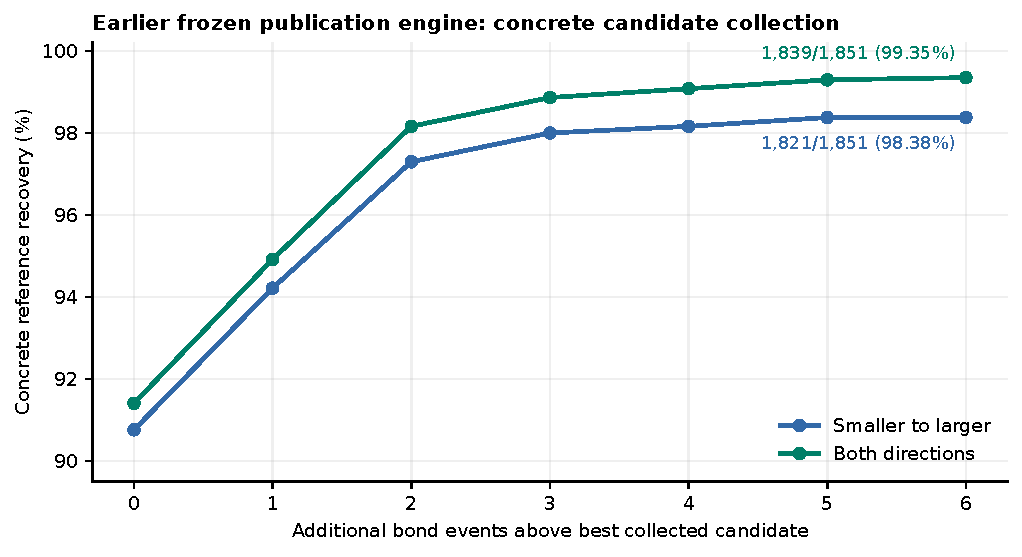
\includegraphics[width=.82\linewidth]{figs/figS2_event_windows.pdf}
\caption{\textbf{Recovery among collected concrete candidates.} This uses the earlier publication engine, separately from the seed ablation. Event windows are relative to the best collected score at maximum coverage. All 1,851 records remain in the denominator. Extraction does not enumerate every represented mapping.}
\label{fig:windows}
\end{figure}

\subsection{Adaptive no-sweep search: a separate policy}
\label{sec:adaptive}
This experiment uses revision \texttt{0ce0f17} and one CPU per direction. A balanced seed agenda uses saved budgets of 400, 1,600, and 6,400 growth operations and a 30 CPU-second soft limit per direction. It retains the native growth cap of 100 but replaces the synchronized frontier cap with an agenda budget. Its last saved checkpoint defines output. Budget completion does not imply agenda exhaustion or successful symbolic verification.

The separate adaptive no-sweep policy verifies 1,723/1,851 Golden references (93.08\%) bidirectionally, with 33 verified absences and 95 unknowns. All 3,702 directional Golden searches complete under their budgets. On the 140 coordinate pairs, it returns full mappings for every case and matches the original ten-order sweep's best saved score in 138 cases; two scores are worse. Thus high mapping availability and score agreement on coordinate inputs do not establish equivalent reference recovery or retained families. This experiment does not isolate the effect of removing cuts from the original scheduler.

\subsection{Accounting scopes}
Across all Golden records, fresh one-, two-, and three-order searches consume 27,084.86, 49,161.91, and 70,570.73 instrumented CPU-seconds. Holdout totals are 1,475.45, 2,417.94, and 3,348.29 seconds. Full-workload totals differ from the common subset.

Completed SLAP sweep calls consume 14.479 CPU-hours of native mapping; mapping plus preparation and export uses 14.934 CPU-hours. Interrupted calls lack final readings. Scheduler TotalCPU fields cannot recover missing consumption on this cluster. Neither these totals nor reserved CPU-hours establish actual total campaign CPU. Mapping spans 8 minutes 9 seconds and separate evaluation spans 35 seconds under allocations different from GRAFT's. These spans are not a matched-latency comparison.

\subsection{Holdout follow-ups}
At tolerance 1.0 and cap 100, case 123 has no full R-to-P output and a 19-event P-to-R representative. Its separate cap-200 follow-up returns a three-event mapping, yielding 134 score ties, six GRAFT-lower cases, and no SLAP-lower cases. Substitution changes SLAP-class membership from 159 represented, 12 excluded, and five unknown to 160 represented, 11 excluded, and five unknown. It is excluded from the fixed-cap panels.

Earlier tolerance-0.5 and proposal-guided studies use distinct policies. In an exploratory uncut holdout ablation, one random ordering matches the full-search best score in 133/140 cases and ten orderings in 138/140. These are score-agreement observations, not Golden accuracy or proof of family equivalence.

\subsection{Supplementary animations}
\textbf{Movie 1: continuous growth and retained placements.}
Carbocation example \texttt{pr16.carbocation\_ts5} (case 64) displays actual extension events and two terminal representatives from an uncut, one-order replay. Changing assignments reflect candidate refinement, not physical reaction motion.

\textbf{Movie 2: deferred boundaries and successive fragments.}
TEMPO example \texttt{pr1.tempo\_ts10} (case 1) follows first-branch events through four fragment decisions and eight deferred-edge observations. A deferred boundary is search evidence, not automatically a chemically broken bond.

The standalone HTML viewer provides playback, event scrubbing, sampled witnesses, terminal selection, H display, and coordinate rotation. Extension views sample at most five witnesses, without enumerating all compressed assignments. Inputs, events, frozen source hashes, and the bookkeeping-binary hash accompany the figure data.
